
\label{section:results}

\begin{table*}[t!]
\centering
\begin{tabular}{c|c|c|c|c|c|c|c|c|c} 
Name    & Version & lines of C code & N(BBs)     & N(BBu)   &  N(DUA) & N(ATP) & Potential Bugs & \% Tested & Yield \\\hline
file    & 5.22    & 12927           & 5694004    & 21141    & 673     & 117    & 19261          & 100\%     & 0.367  \\
eog     & 3.4.2   & 22997           & ?          &          &         &        &                &           & \\
bash    & 4.3     & 98871           & ?          &          &         &        &                &           & \\
readelf & 2.25    & 1327513         & 8131559    & 21399    & 3875    & 266    & 276855         & 0.1\%     & 0.0303 \\
tshark  & 1.8.2   & 2186252         & 304741643  & 207273   & 9765    & 1035   & 1224297        & 0.01\%    & 0.125 \\
\end{tabular}
\caption{Injection results for open source programs of various sizes.
For each, a single input file was used to perform a taint analysis with PANDA.
Various program and dynamic trace statistics are reported as well as DUA, attack point (ATP), and yield (fraction of injected bugs that result in a segmentation violation).}
\end{table*}

We evaluated VITAL in three ways.
First, we injected large numbers of bugs into five open source programs: file, readelf (from binutils), bash, tshark (command-line verison of Wireshark), and eog (aka Eye of GNOME, an image viewer).
For each of these, we report various statistics with respect to both the target program and also VITAL's success at injecting bugs.
Second, we propose and compute some measures of how realistic these bugs are.
Third, we randomly sampled 20 injected bugs for each of these programs and used these to measure detection rates for two commercial and two open source bug finders.

\subsection{Injection Experiments}



The results of injecting bugs into open source programs are summarized in Table~\ref{table:open-source-targets}.
In this table, programs are ordered by size, in lines of C code, as measured by David Wheeler's \verb+sloccount+.  % \footnote{For \verb+readelf+ and \verb+tshark+, we report lines of code for the larger projects which contain them: binutils and Wireshark, as they are not easily extricable }.
A single input was used with each program to measure taint and find injectable bugs.
The input to \verb+file+ and \verb+readelf+ was the program \verb+ls+.
The input to \verb+tshark+ was a single iptrace [from brendan -- where did \verb+dualhome.iptrace+ come from?]. 
The input to \verb+eog+ was ...
The input to \verb+bash+ was ...
The number of sequential and unique basic blocks in the PANDA trace for each program are reported as N(BBs) and N(BBu).
N(DUA) and N(ATP) are the number of DUAs and attack points collected in the VITAL database by the FIB analysis.
Note that, in order for a DUA or attack point to be counted, it must have been deemed viable for some bug (each bug is a DUA-ATP pair) [is this well explained elsewhere?]

Exhaustive testing was not possible for all programs.  
Larger targets had larger numbers of potential bugs: over a million for \verb+tshark+.
Further, larger targets take longer to test: about 11 minutes for\verb+tshark+.
This is because testing requires not only injecting a small amount of code to add the bug, but also recompiling and running.
For the larger programs like readelf and tshark, we found the build to be subtly broken so that a \verb+make clean+ was necessary to pick up the bug injection reliably.
Thus, we were only able to test about 1000 potential bugs for each of the two largest programs. 
[Should we have a column for testing time by program?  ~10 sec for file.  ~9 min for readelf.  ~11 min for tshark]
The type of bug injected was an out-of-bounds pointer use (either read or write) as described in Section X.
As the bug is designed to be triggered only if a particular set of four bytes in the input contain the characters 'vital',
we tested with both the original input and with the fuzzed one that contained the trigger. 
We did not encounter any situation in which the original input caused a segfault [is that true?].

The final column in Table~\ref{table:open-source-targets} reports yield, which is the fraction of potential bugs that were tested and found to actually segfault.
This number varies considerably from a few percent to almost forty percent.
To understand this, we investigated the relationship between our two taint-based measures and yield.
For each DUA used to inject a bug, we determined the maximum TCN for any of its bytes and the maximum liveness for any label in any taint set associated with one of its bytes.  
More informally, the first of these two quantities, $mTCN$, represents how complicated a function of the input bytes a DUA is.
The second, $mLIV$, is a measure of how much the control flow of a program is influenced by the input bytes that determine a DUA.
Table~\ref{table:yield-breakdown} explores the relationship between yield and these two quantities. 
This table is really a two-dimensional histogram, with the top-left cell representing all bug injections for which $mTCN=mLIV=0$, and the bottom-right cell being all those for which $mTCN>=100$ and $mLIV>=100$
When $mTCN=mLIV=0$, the DUA is a direct copy of input bytes and none of those input bytes are used to decide any program branches, and yield is 0.526.
As either $mTCN$ or $mLIV$ increase, yield deteriorates.  

\begin{table}
\centering
\begin{tabular}{l|l|l|l|l} 
 & \multicolumn{3}{c}{mLIV} &  \\  
$mTCN$ &         $[0,1)$ & $[1,10)$ & $[10,100)$ & $[100,+\inf]$ \\  \hline 
$[0,1)$ &       0.526   & 0.466    & 0.208      & 0.218 \\
$[1,10)$ &      --      & 0.119    & --         & --    \\
$[10,100)$ &    --      & --       & 0.000      & --    \\
$[100,+\inf]$ & --      & --       & --         & -- \\ 
\end{tabular}
\caption{Yield as a function of both mLIV and mTCN.  
Yield is highest for DUAs that are both an uncomplicated function of input bytes, and that do no derive from input bytes that are used to decide program control flow.}
\label{table:open-source-targets}
\end{table}


\subsection{Bug Realism}

\begin{figure}
\centering
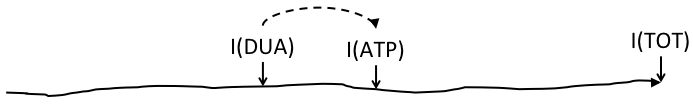
\includegraphics[width=3in]{trace-dua-atp.png}
\caption{A cartoon representing an entire program trace, annotated with instructions at which DUA is siphoned off to be used, I(DUA), attack point where it is used, I(ATP), and total number of instructions in trace, I(TOT).}
\label{fig:dua-atp-trace}
\end{figure}

The intended use of the bugs created by this system is as ground truth for development and evaluation of vulnerability injection schemes.
Thus, it is crucial that they be realistic in some sense.  
Realism is, however, not easy to assess.
We examined three aspects of our injected bugs as measures of realism. 
The first two are DUA and attack point position within the program trace, which are depicted in Figure~\ref{fig:dua-atp-trace}.
That is, we determined the fraction of trace instructions executed at the point the DUA is siphoned off and at the point it is used to attack the program by corrupting a pointer.
Histograms for these two quantities, $I(DUA)$ and $I(ATP)$, are provided in Figures~\ref{fig:dua-hist} and~\ref{fig:atp-hist}, where counts are for all potential bugs in the VITAL database for all five open source programs. 
DUAs and attack points are clearly available at all points during the trace, although there appear to be more at the beginning and end.
This is important, since bugs created using these DUAs have entirely realistic control and data-flow all the way up to $I(DUA)$.
Therefore, vulnerability discovery tools will have to reason correctly about all of the program up to $I(DUA)$ in order to correctly diagnose the bug.
The portion of the trace \emph{between} the $I(DUA)$ and $I(ATP)$ is of particular interest since, currently, VITAL makes data flow between DUA and attack point via a pair of function calls.
Thus, it might be argued that this is an unrealistic portion of the trace in terms of data flow.
The quantity $I(DUA)/I(ATP)$ will be close to 1 for injected bugs that minimize this source of unrealism.
This would correspond to the worked example in Figure~\ref{fig:worked-example}; the DUA is still in scope, when, a few lines later in the same function, it can be used to corrupt a pointer.
No abnormal data flow is required.
The histogram in Figure~\ref{fig:rdf-hist} quantifies this effect for all potential VITAL bugs, and it is clear that a large fraction have $I(DUA)/I(ATP) \approx 1$, and are therefore highly realistic.

\begin{figure}
\centering
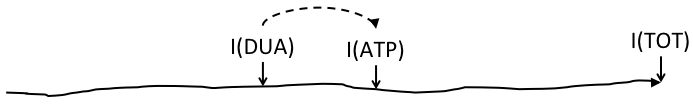
\includegraphics[width=3in]{trace-dua-atp.png}
\caption{A cartoon representing an entire program trace, annotated with instructions at which DUA is siphoned off to be used, I(DUA), attack point where it is used, I(ATP), and total number of instructions in trace, I(TOT).}
\label{fig:taint-compute-number}
\end{figure}

\begin{figure}
\centering
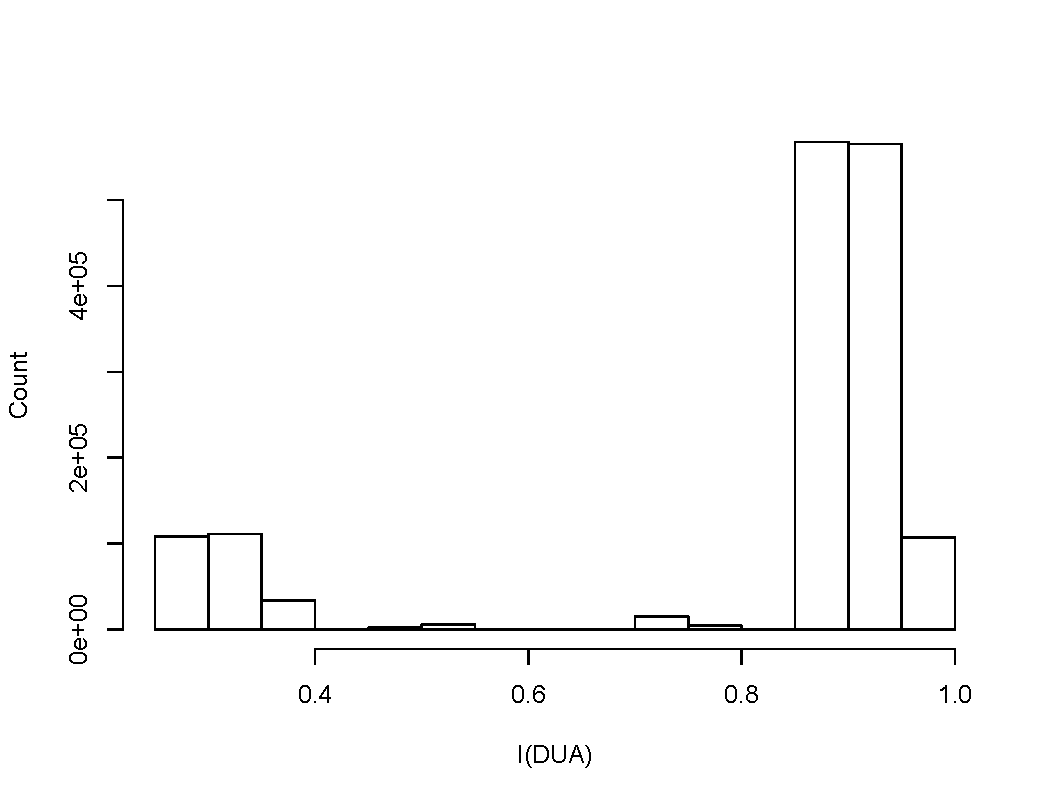
\includegraphics[width=3in]{dua.pdf}
\caption{Normalized DUA trace location}
\label{fig:dua-hist}
\end{figure}

\begin{figure}
\centering
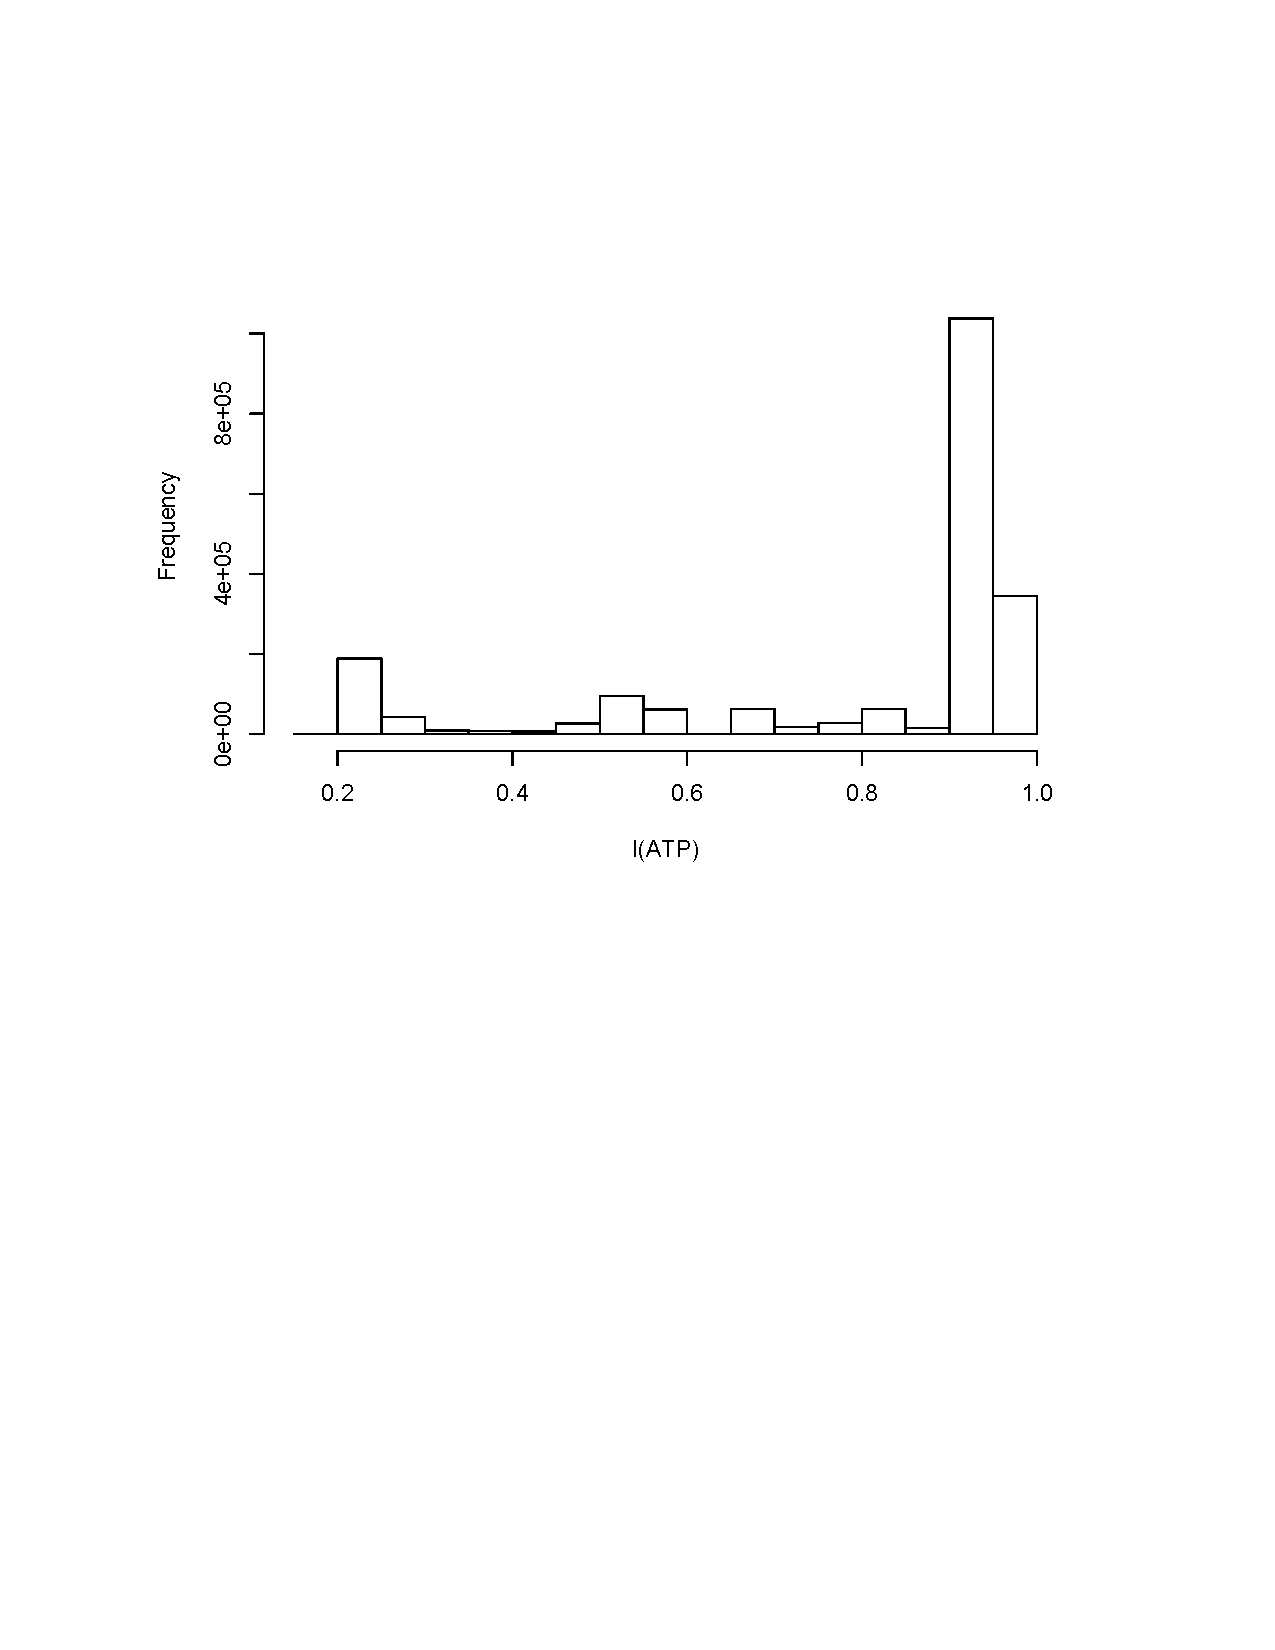
\includegraphics[width=3in]{atp.pdf}
\caption{Normalized DUA trace location}
\label{fig:atp-hist}

\end{figure}
\begin{figure}
\centering
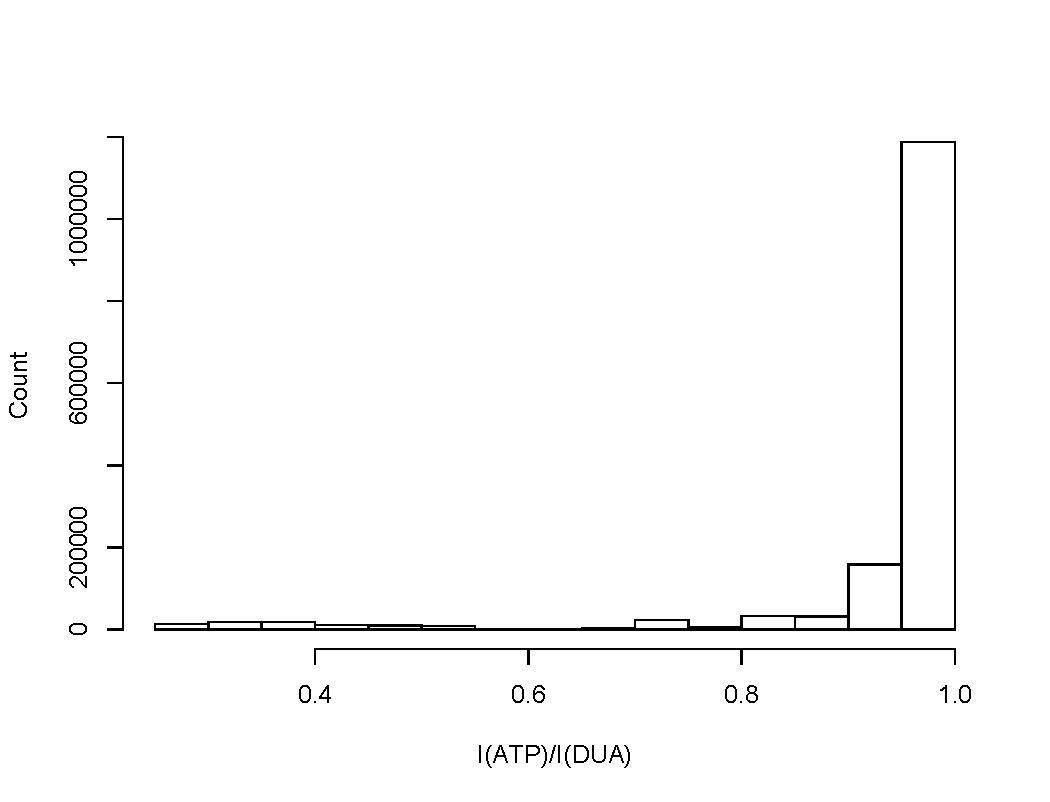
\includegraphics[width=3in]{rdf.pdf}
\caption{Fraction of trace with perfectly normal or realistic data flow, $I(DUA)/I(ATP)$}
\label{fig:rdf-hist}
\end{figure}




